% !TEX root = ../MasterThesis_goto_v1.tex

%%%%%%%%%%%%%%%%%%%%%%%%%%%%%%%%%%%%%%%%%%%%%%%%%%%%%%%%%%%%%%%%%%%%%%%%%%%%%%%%%%%%%%%%%%%%%%%%%%%%%
\chapter{崩壊点検出の為のネットワーク} \label{chap:Networks}

\ref{chap:Networks}章と\ref{chap:VertexFinderwithDL}章、\ref{chap:Comparison}章は本論文の本題である。
\ref{chap:Networks}章では本研究で使用するデータと深層学習のネットワークについて、\ref{chap:VertexFinderwithDL}章では\ref{chap:Networks}章で作成したネットワークを用いた崩壊点検出について、\ref{chap:Comparison}章ではその様にして作成した崩壊点検出と現行の崩壊点検出との比較について、それぞれ解説する。

本章では、まず\ref{Net:Data}節で本研究で取り扱うデータの性質について述べる。
次に、\ref{Net:forVertexFinderwithDL}節にて深層学習を使用した崩壊点検出をどのように実現するかについて概要を説明する。
個々のネットワークの詳細な構造や学習、ネットワーク単体での性能については\ref{Net:PairModel}節、\ref{Net:VertexLSTM}節で解説する。
これらネットワークについては\ref{chap:DeepLearning}章の内容を前提とし、訓練データ、ハイパーパラメーター・チューニングについてもここで述べる。

%%%%%%%%%%%%%%%%%%%%%%%%%%%%%%%%%%%%%%%%%%%%%%%%%%%%%%%%%%%%%%%%%%%%%%%%%%%%%%%%%%%%%%%%%%%%%%%%%%%%%
\section{データ} \label{Net:Data}

ここでは、本研究で使用したモンテカルロシミュレーションデータについて述べる。
特に\ref{Net:Data:DataProperty}項では、データ全体についての性質に関して、\ref{Net:Data:TrackInformationandPreprocessing}項では、本研究で使用する飛跡についての情報と前処理について詳しく述べる。
ただし、各ネットワークの学習に使用する訓練データの詳細に関しては、後の\ref{Net:PM:TrainingandStrategyofPM}や\ref{Net:VLSTM:TrainingandStrategyofVLSTM}で紹介する。

%%%%%%%%%%%%%%%%%%%%%%%%%%%%%%%%%%%%%%%%%%%%%%%%%%%%%%%%%%%%%%%%%%%%%%%%
\subsection{データ全体の性質} \label{Net:Data:DataProperty}

どのようなシミュレーションソフトを使っているか。\\
エネルギー・終状態・Tertiary Vertex・イベント毎の飛跡の数・崩壊点の種類と割合・(後述する)本数個数が異なる

%%%%%%%%%%%%%%%%%%%%%%%%%%%%%%%%%%%%%%%%%%%%%%%%%%%%%%%%%%%%%%%%%%%%%%%%
\subsection{飛跡の情報と前処理} \label{Net:Data:TrackInformationandPreprocessing}

各変数について・Helix parametersの定義\cite{TrackParametersLCIO}
Helix parametersの元の分布やreshape後の分布について\\

%%%%%%%%%%%%%%%%%%%%%%%%%%%%%%%%%%%%%%%%%%%%%%%%%%%%%%%%%%%%%%%%%%%%%%%%%%%%%%%%%%%%%%%%%%%%%%%%%%%%%
\section{深層学習を用いた崩壊点検出の実現} \label{Net:forVertexFinderwithDL}

深層学習ができること。分類・回帰問題に落とし込むという事。\\
気をつけねばならないこと。データの性質にあったネットワークが必要である。今回取り扱うデータにおいて、\\

以上を踏まえた上で私は二つのネットワークを用いた崩壊点検出を提案する。\\
一つはーーーを用いて、崩壊点の種類と位置の予測を行う為のネットワークである。\\
もう一つはーーーーとーーーーを用いて、ーーーーを行う為のネットワークである。\\
詳細なネットワークの構造については、後の\ref{Net:PairModel}、\ref{Net:VLSTMModel}節で述べる。\\
二つあって、何をして、入力と出力、ネットワークを作る上での技術\\
訓練データの作り方・ハイパーパラメータの標準は「ネットワークの構造」\\

これらのネットワークはーーーーを用いて実装した。\\
tensorflow・keras・TITAN RTX・ITO\\


%%%%%%%%%%%%%%%%%%%%%%%%%%%%%%%%%%%%%%%%%%%%%%%%%%%%%%%%%%%%%%%%%%%%%%%%%%%%%%%%%%%%%%%%%%%%%%%%%%%%%
\section{飛跡対についてのネットワーク} \label{Net:PairModel}

ここでは\ref{Net:forVertexFinderwithDL}節で紹介した二つのネットワークの内、飛跡対のためのネットワークについて述べる。
主にネットワークの構造に関しては\ref{Net:PM:StructureofPM}項で、学習に関しては\ref{Net:PM:TrainingandStrategyofPM}項で解説する。
また、そのようにして構築、訓練されたネットワーク単体についての性能と簡単な評価に関しては、\ref{Net:PM:PerformanceofPM}項で述べることとする。

%%%%%%%%%%%%%%%%%%%%%%%%%%%%%%%%%%%%%%%%%%%%%%%%%%%%%%%%%%%%%%%%%%%%%%%%
\subsection{ネットワークの構造} \label{Net:PM:StructureofPM}


\begin{figure}[h]
 \centering
 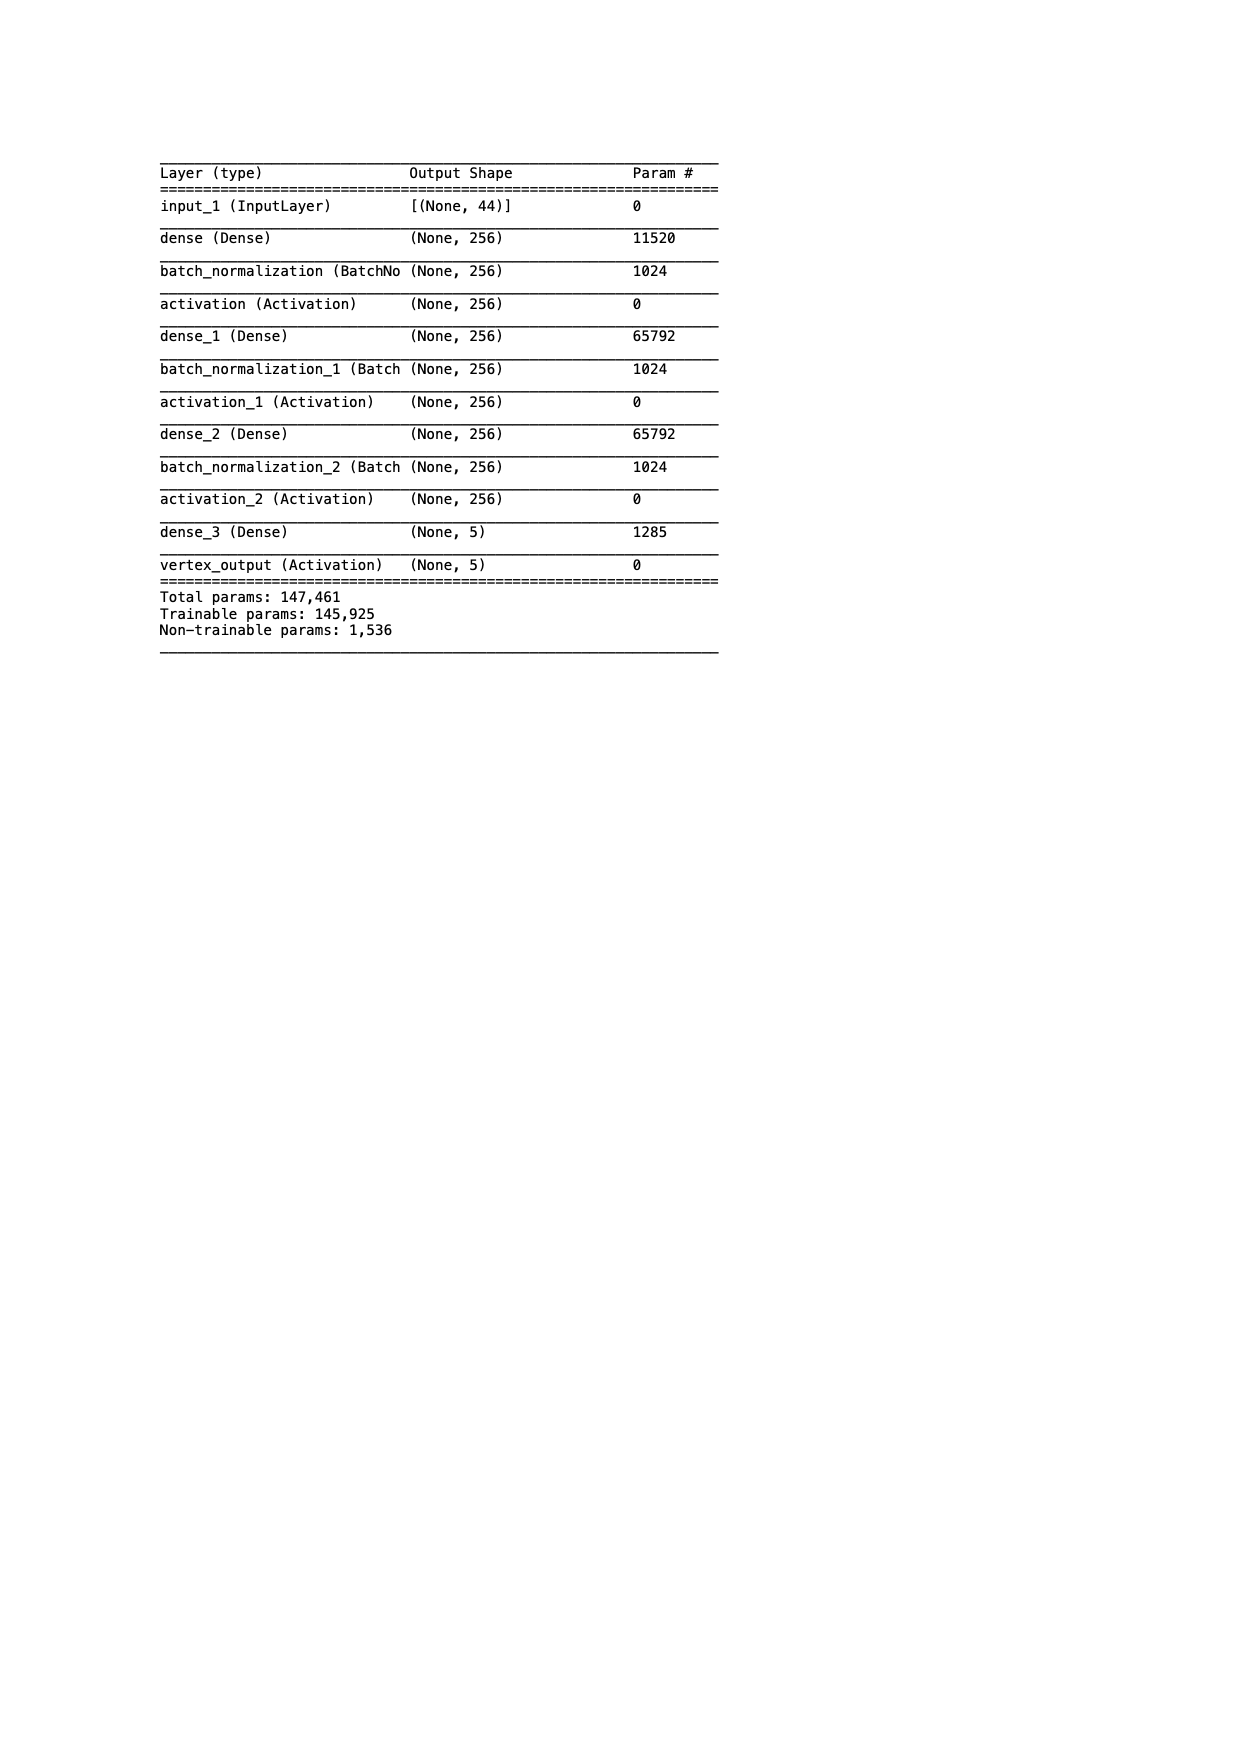
\includegraphics[trim = 0 200 0 200, width=0.9\textwidth]{Figure/3Networks/3-3-1-1PairModelSummary.png}
 \caption{エンコーダー・デコーダーモデルにおける各種パラメーターの出力}
 \label{3-3-1-3VLSTMSummary}
\end{figure}


%%%%%%%%%%%%%%%%%%%%%%%%%%%%%%%%%%%%%%%%%%%%%%%%%%%%%%%%%%%%%%%%%%%%%%%%
\subsection{ネットワークの学習と戦略} \label{Net:PM:TrainingandStrategyofPM}



%%%%%%%%%%%%%%%%%%%%%%%%%%%%%%%%%%%%%%%%%%%%%%%%%%%%%%%%%%%%%%%%%%%%%%%%
\subsection{ネットワークの性能} \label{Net:PM:PerformanceofPM}

%%%%%%%%%%%%%%%%%%%%%%%%%%%%%%%%%%%%%%%%%%%%%%%%%%%%%%%%%%%%%%%%%%%%%%%%%%%%%%%%%%%%%%%%%%%%%%%%%%%%%
\section{任意の数の飛跡についてのネットワーク} \label{Net:VertexLSTM}

ここでは\ref{Net:forVertexFinderwithDL}節で紹介した二つのネットワークの内、任意の数の飛跡のためのネットワークについて述べる。
基本的には前節の飛跡対についてのネットワークと同様の手順での解説を行うが、この任意の数の飛跡についてのネットワークは、既存のネットワーク構造にはない独自のネットワークで構築している。
これは本研究におけるデータの特殊性や問題解決のための最適なネットワークを考慮した結果である。
このようなネットワークの詳細な構造については\ref{Net:VLSTM:DetailedStructureofVLSTM}項で述べる。


%%%%%%%%%%%%%%%%%%%%%%%%%%%%%%%%%%%%%%%%%%%%%%%%%%%%%%%%%%%%%%%%%%%%%%%%
\subsection{ネットワークの構造} \label{Net:VLSTM:StructureofVLSTM}

\begin{figure}[h]
 \centering
 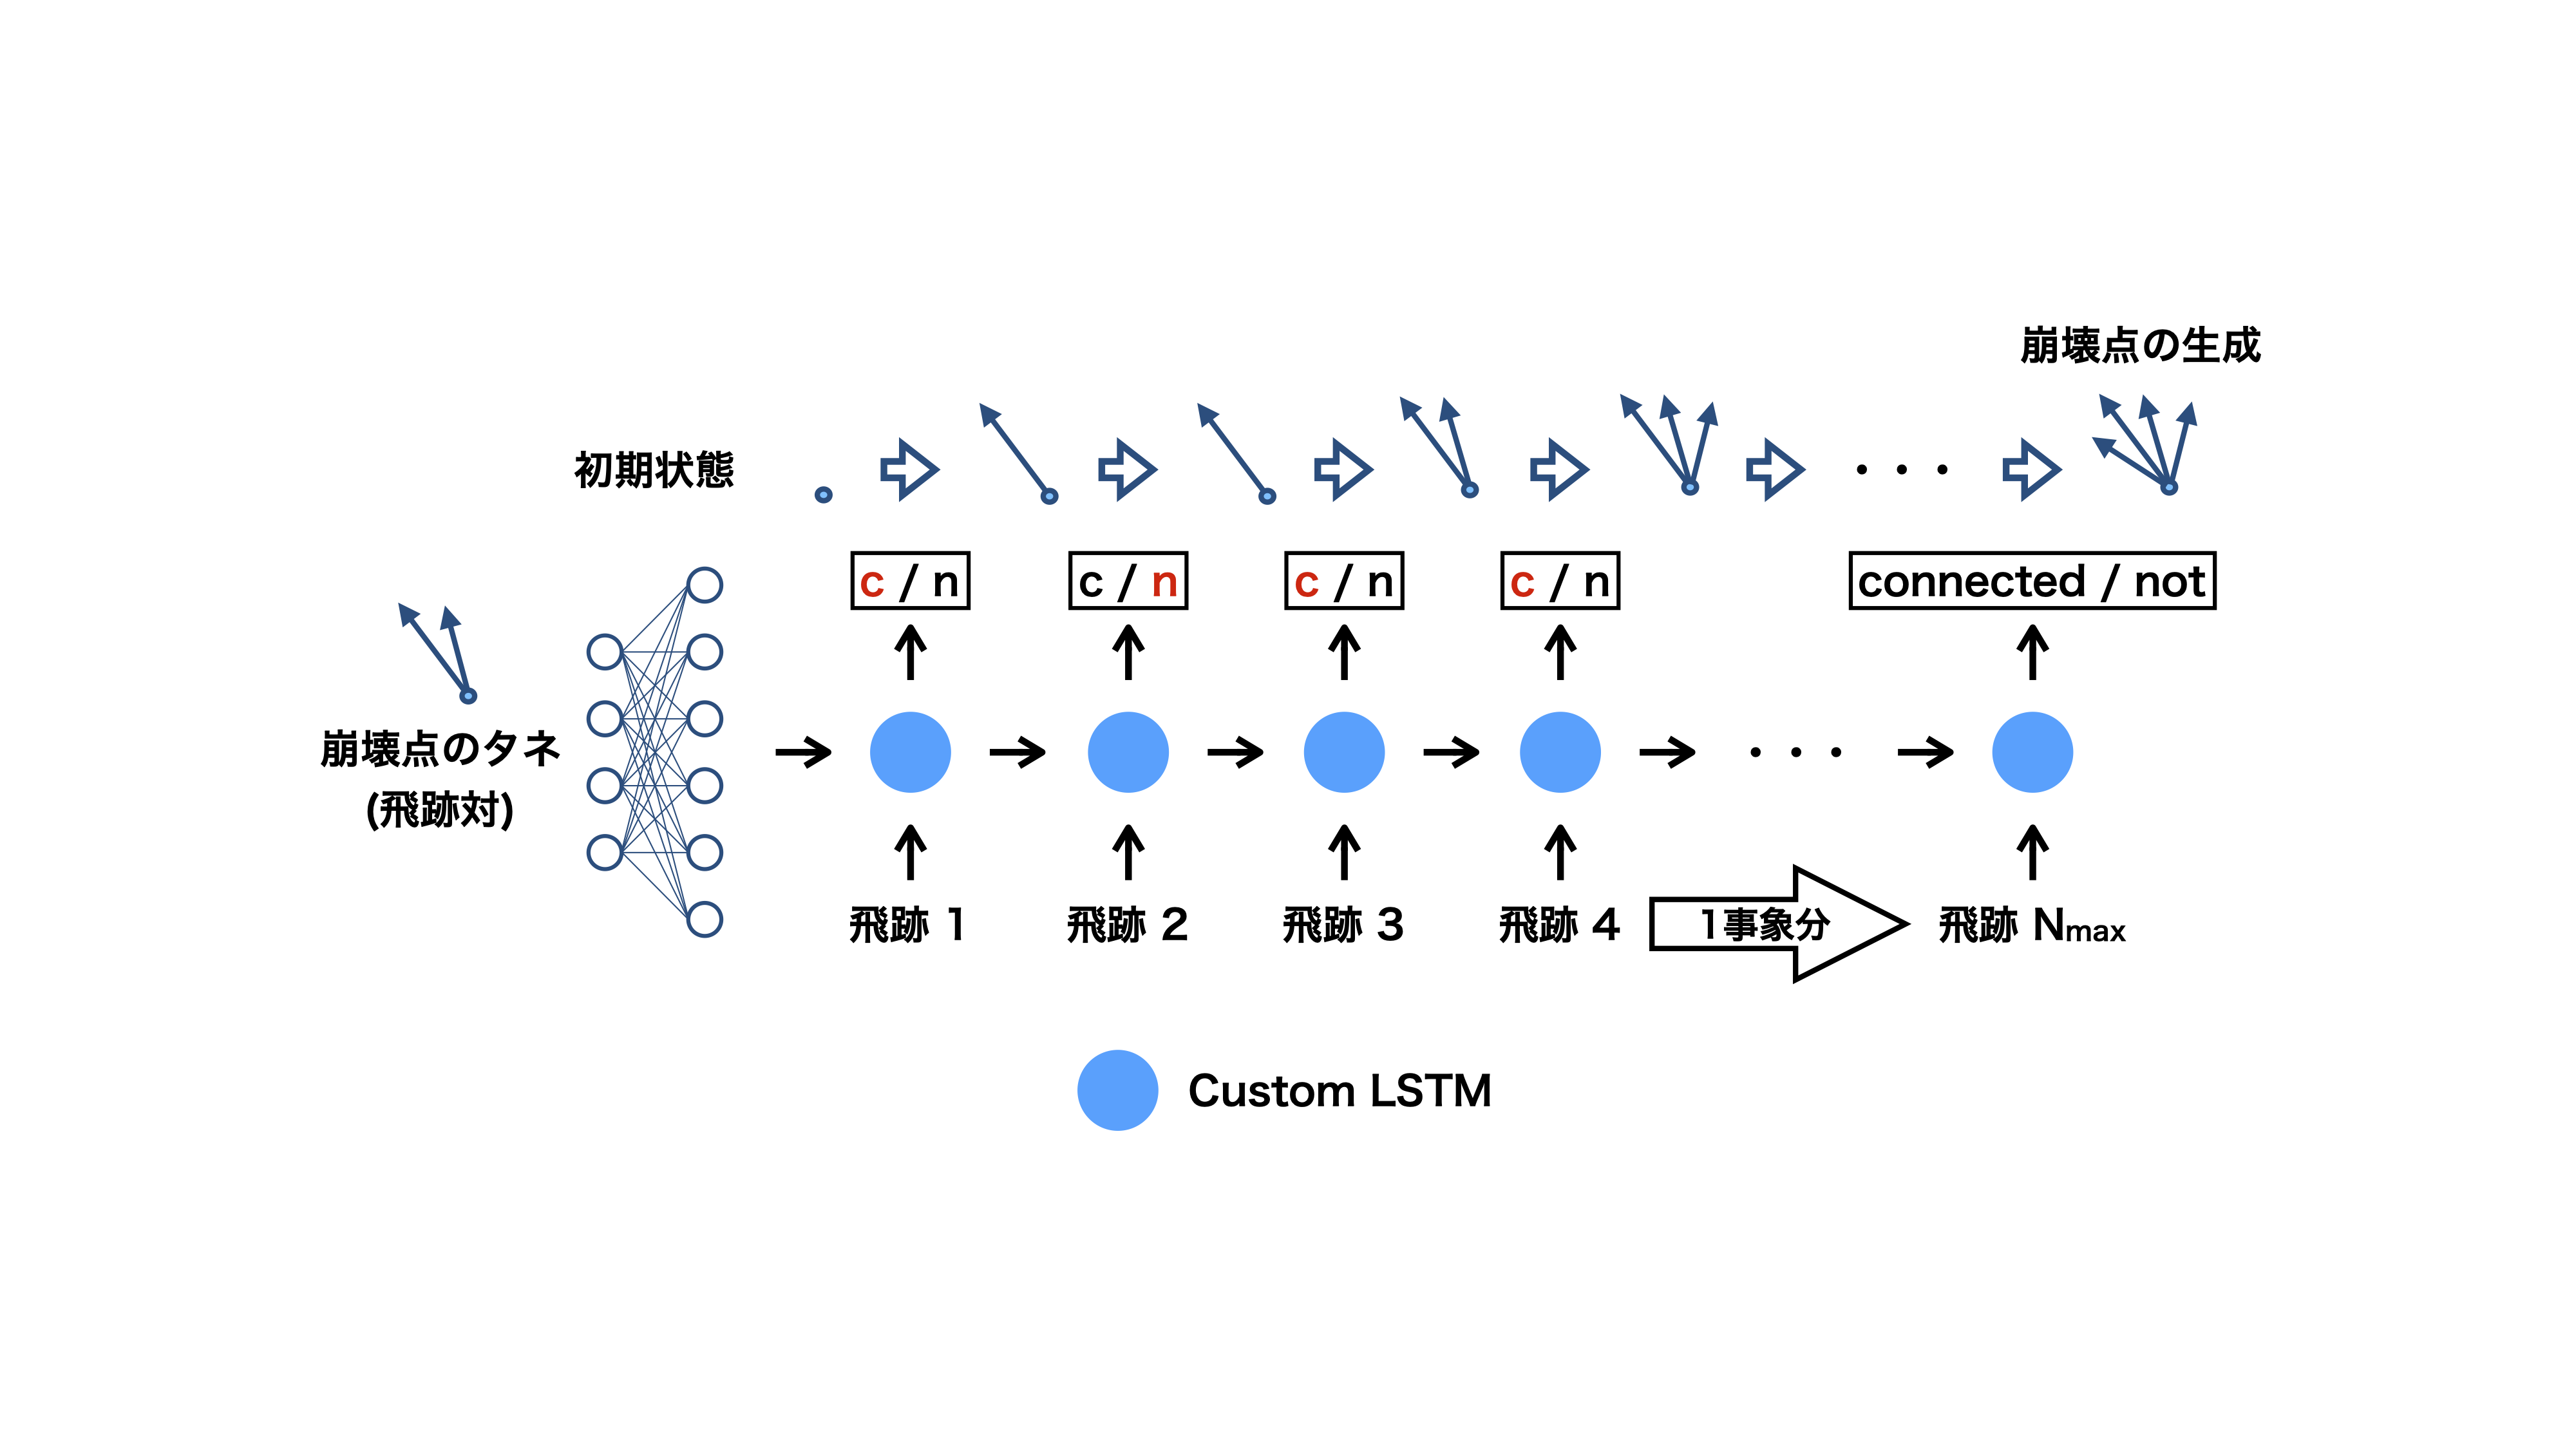
\includegraphics[width=1.0\textwidth]{Figure/3Networks/3-4-1-1SimpleVLSTM.png}
 \caption{自作リカレントニューラルネットワークを用いた崩壊点の生成}
 \label{3-4-1-1SimpleVLSTM.png}
\end{figure}

\begin{figure}[h]
 \centering
 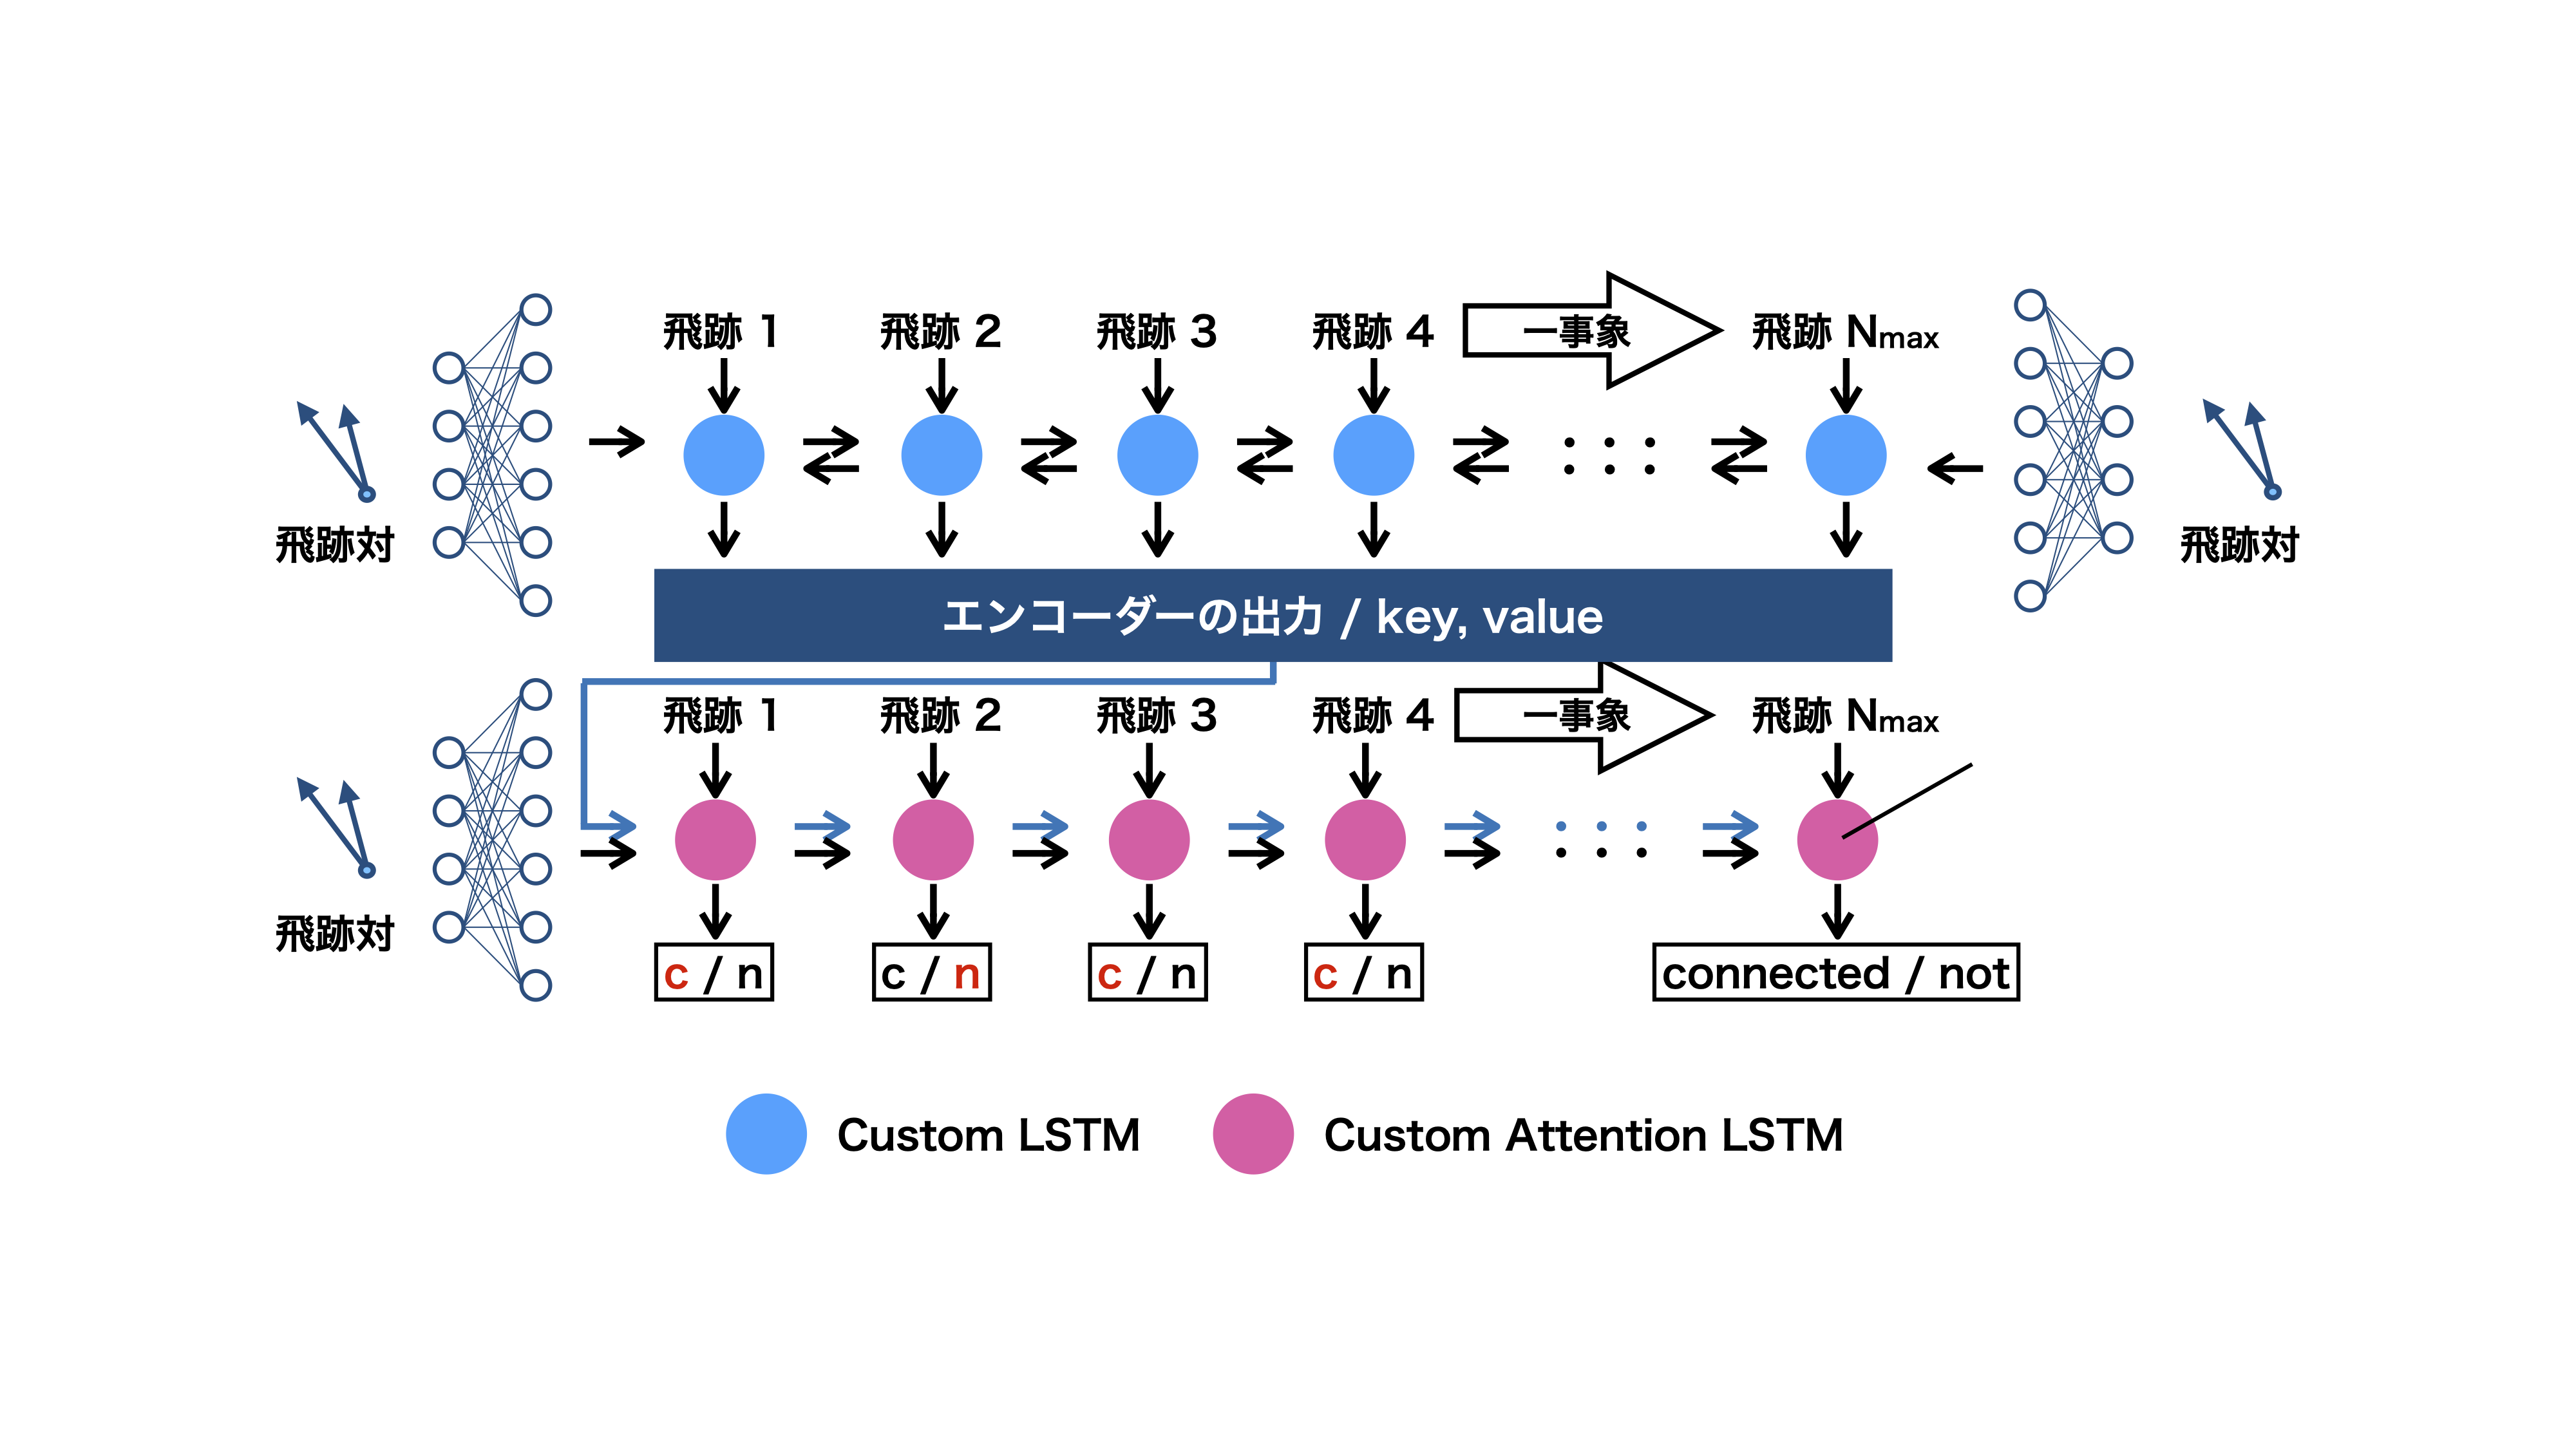
\includegraphics[width=1.0\textwidth]{Figure/3Networks/3-4-1-2EncoderDecoderVLSTM.png}
 \caption{自作リカレントニューラルネットワークのエンコーダー・デコーダーモデルへの拡張}
 \label{3-4-1-2EncoderDecoderVLSTM.png}
\end{figure}

\begin{figure}[h]
 \centering
 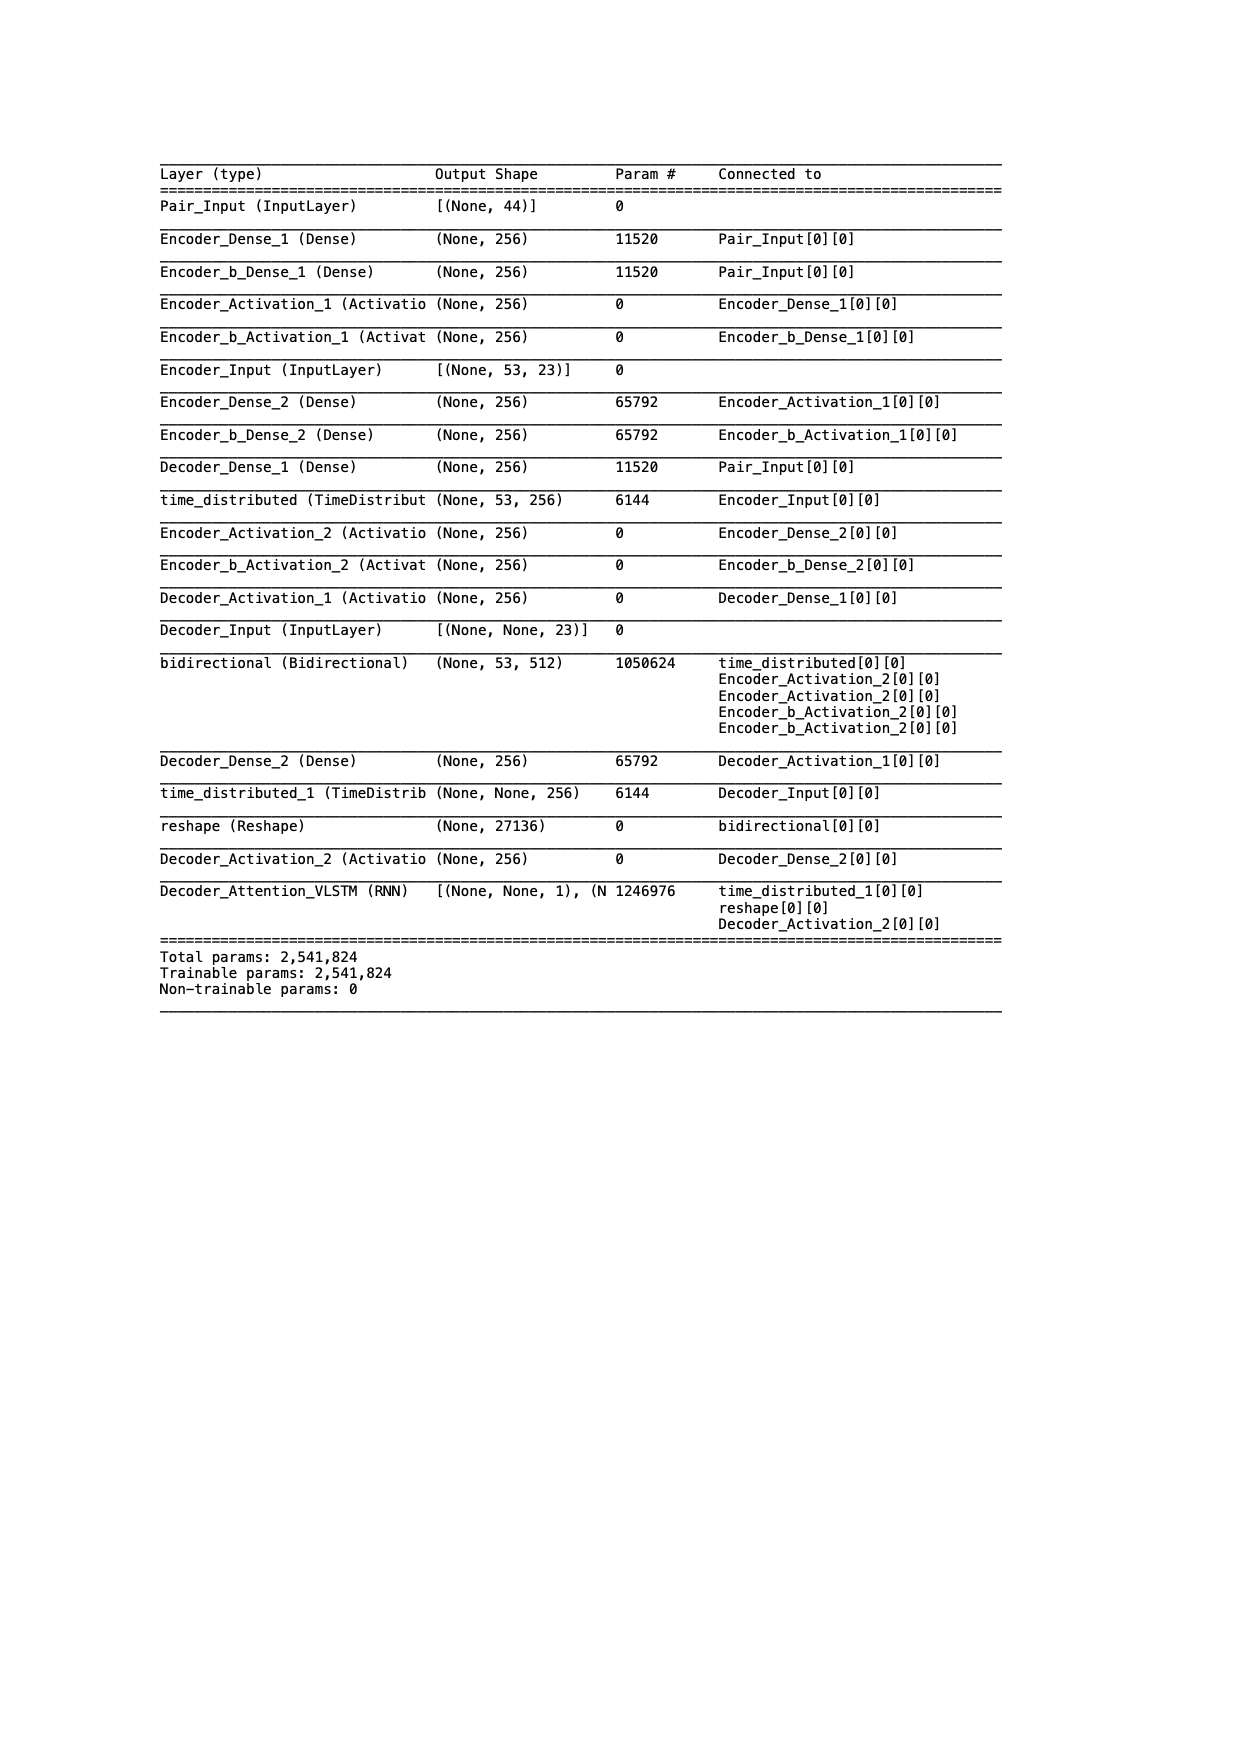
\includegraphics[trim = 0 200 0 200, width=0.9\textwidth]{Figure/3Networks/3-4-1-3VLSTMSummary.png}
 \caption{エンコーダー・デコーダーモデルにおける各種パラメーターの出力}
 \label{3-4-1-3VLSTMSummary}
\end{figure}


%%%%%%%%%%%%%%%%%%%%%%%%%%%%%%%%%%%%%%%%%%%%%%%%%%%%%%%%%%%%%%%%%%%%%%%%
\subsection{ネットワークの詳細な構造} \label{Net:VLSTM:DetailedStructureofVLSTM}

\begin{figure}[h]
 \centering
 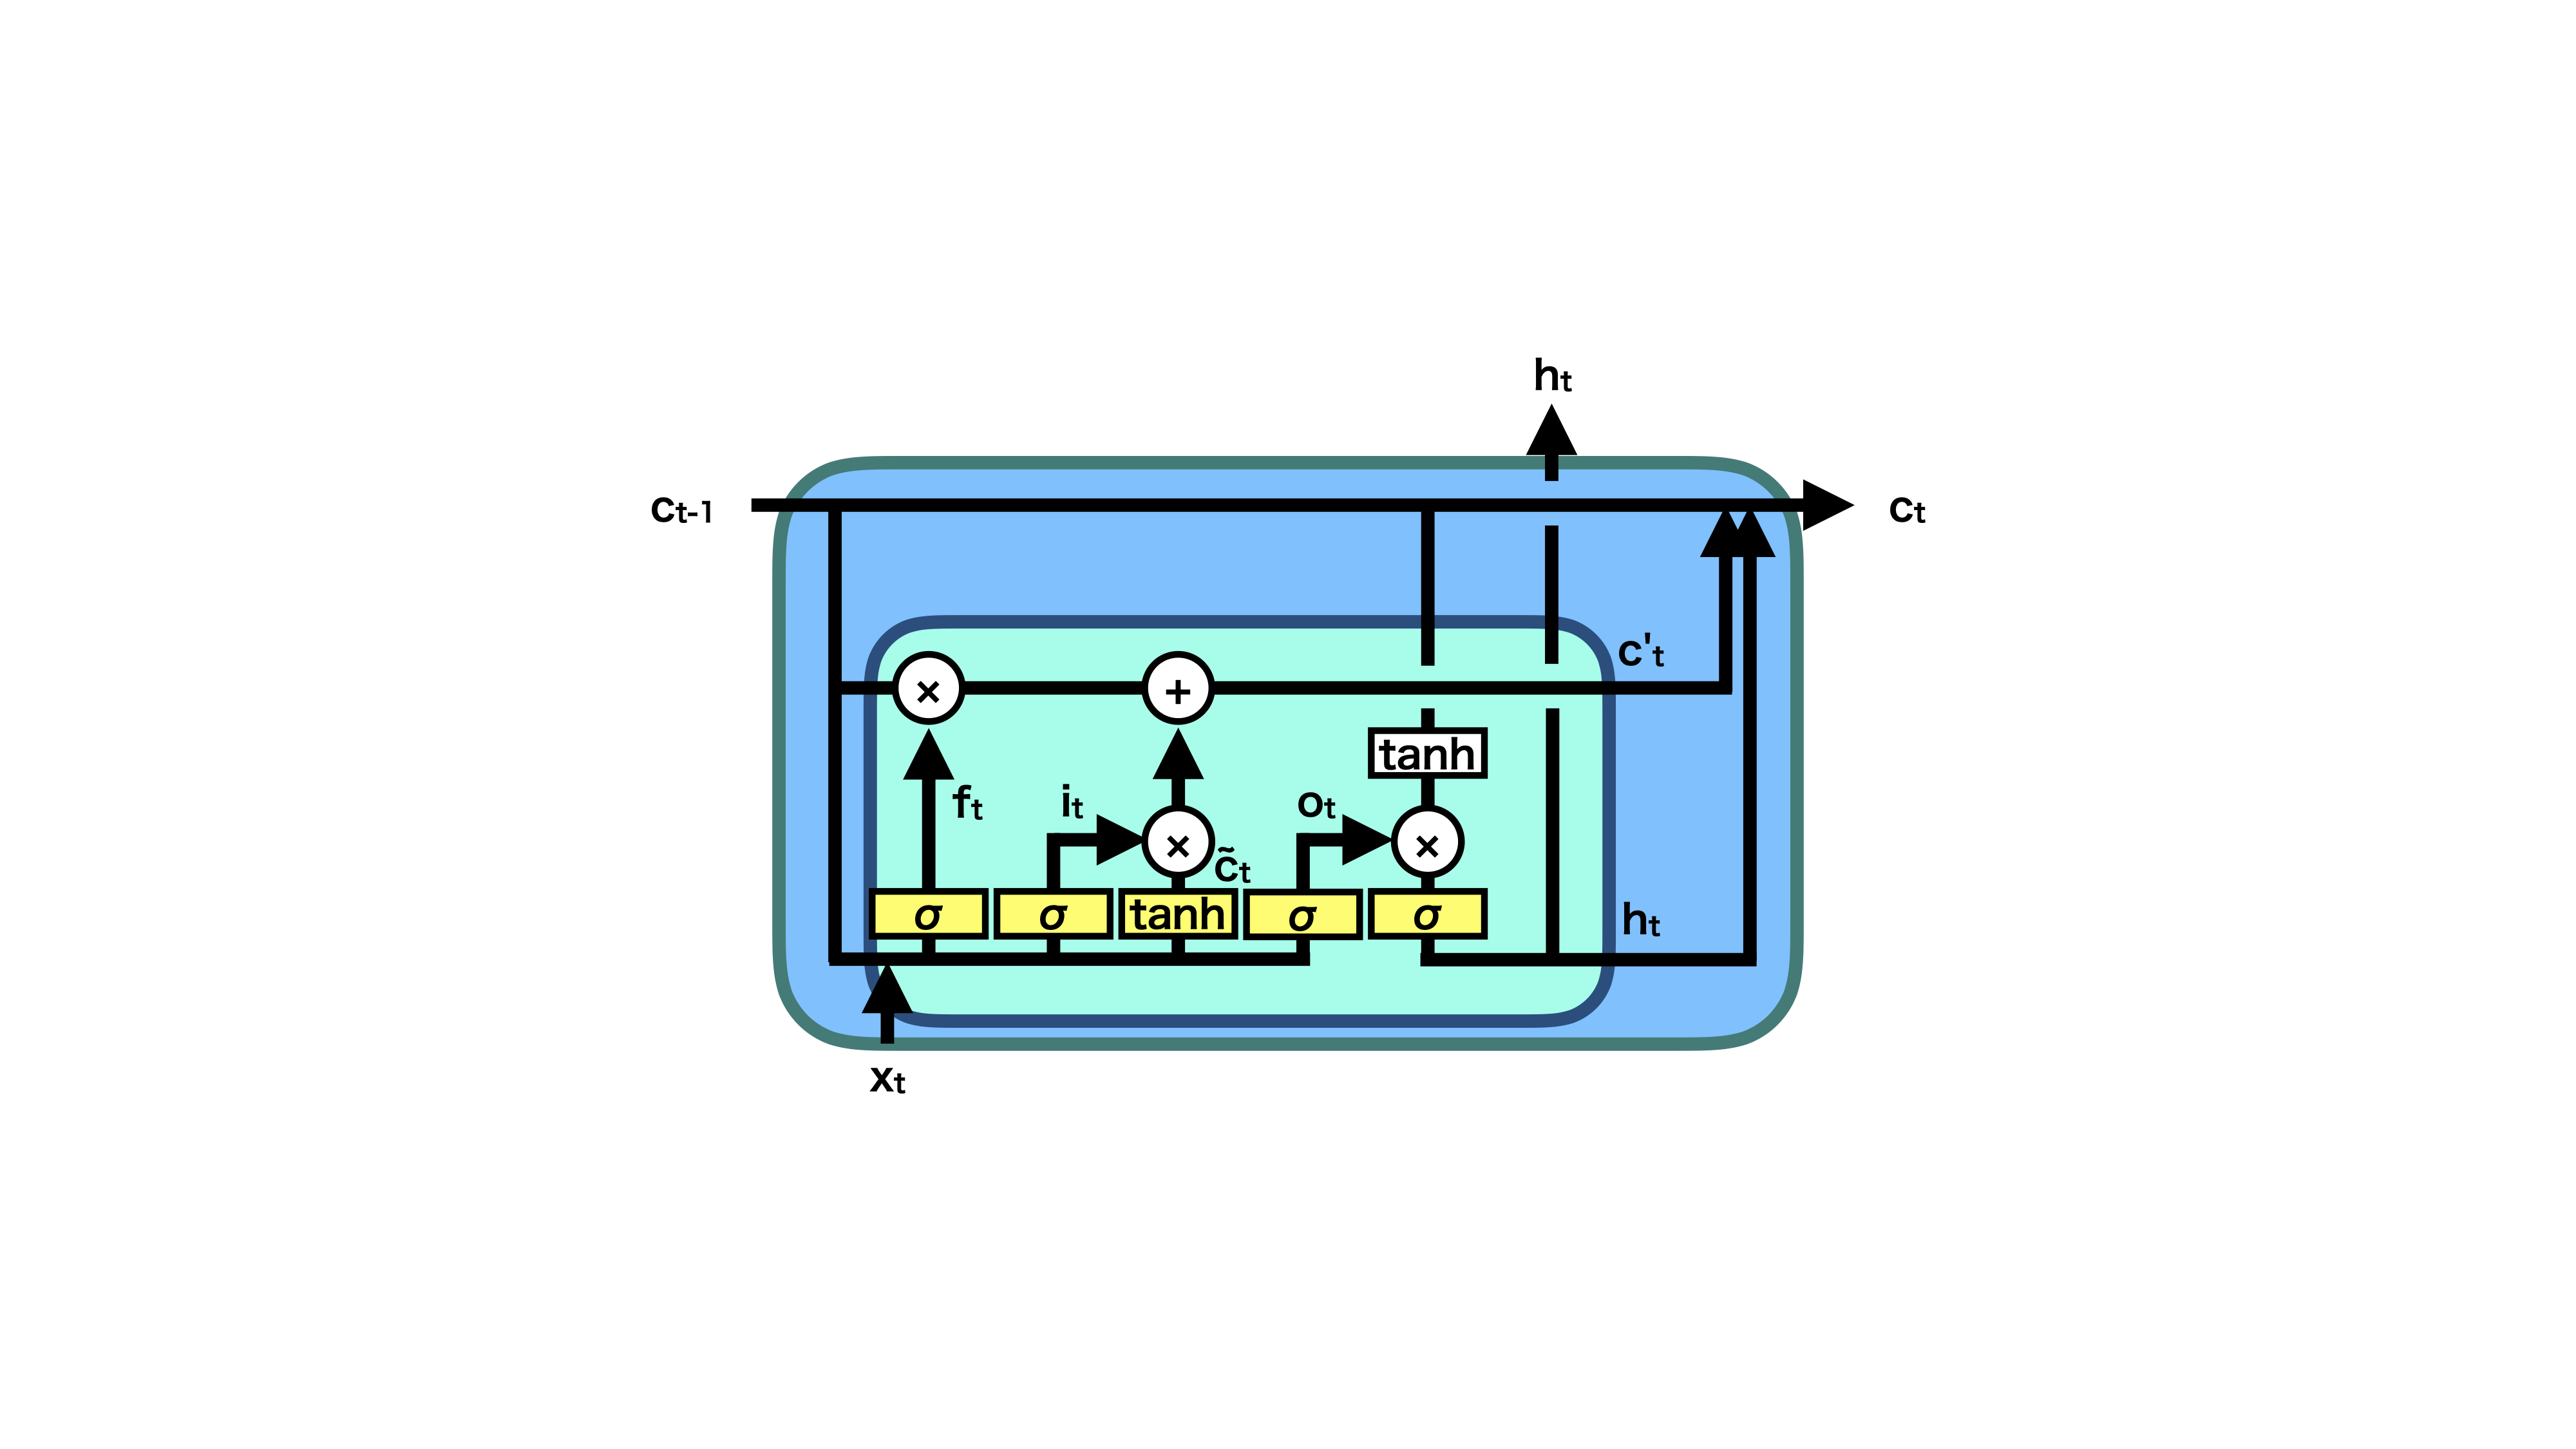
\includegraphics[width=0.9\textwidth]{Figure/3Networks/3-4-2-1VLSTMStructure.png}
 \caption{自作リカレントニューラルネットワークの構造}
 \label{3-4-2-1VLSTMStructure}
\end{figure}

\begin{figure}[h]
 \centering
 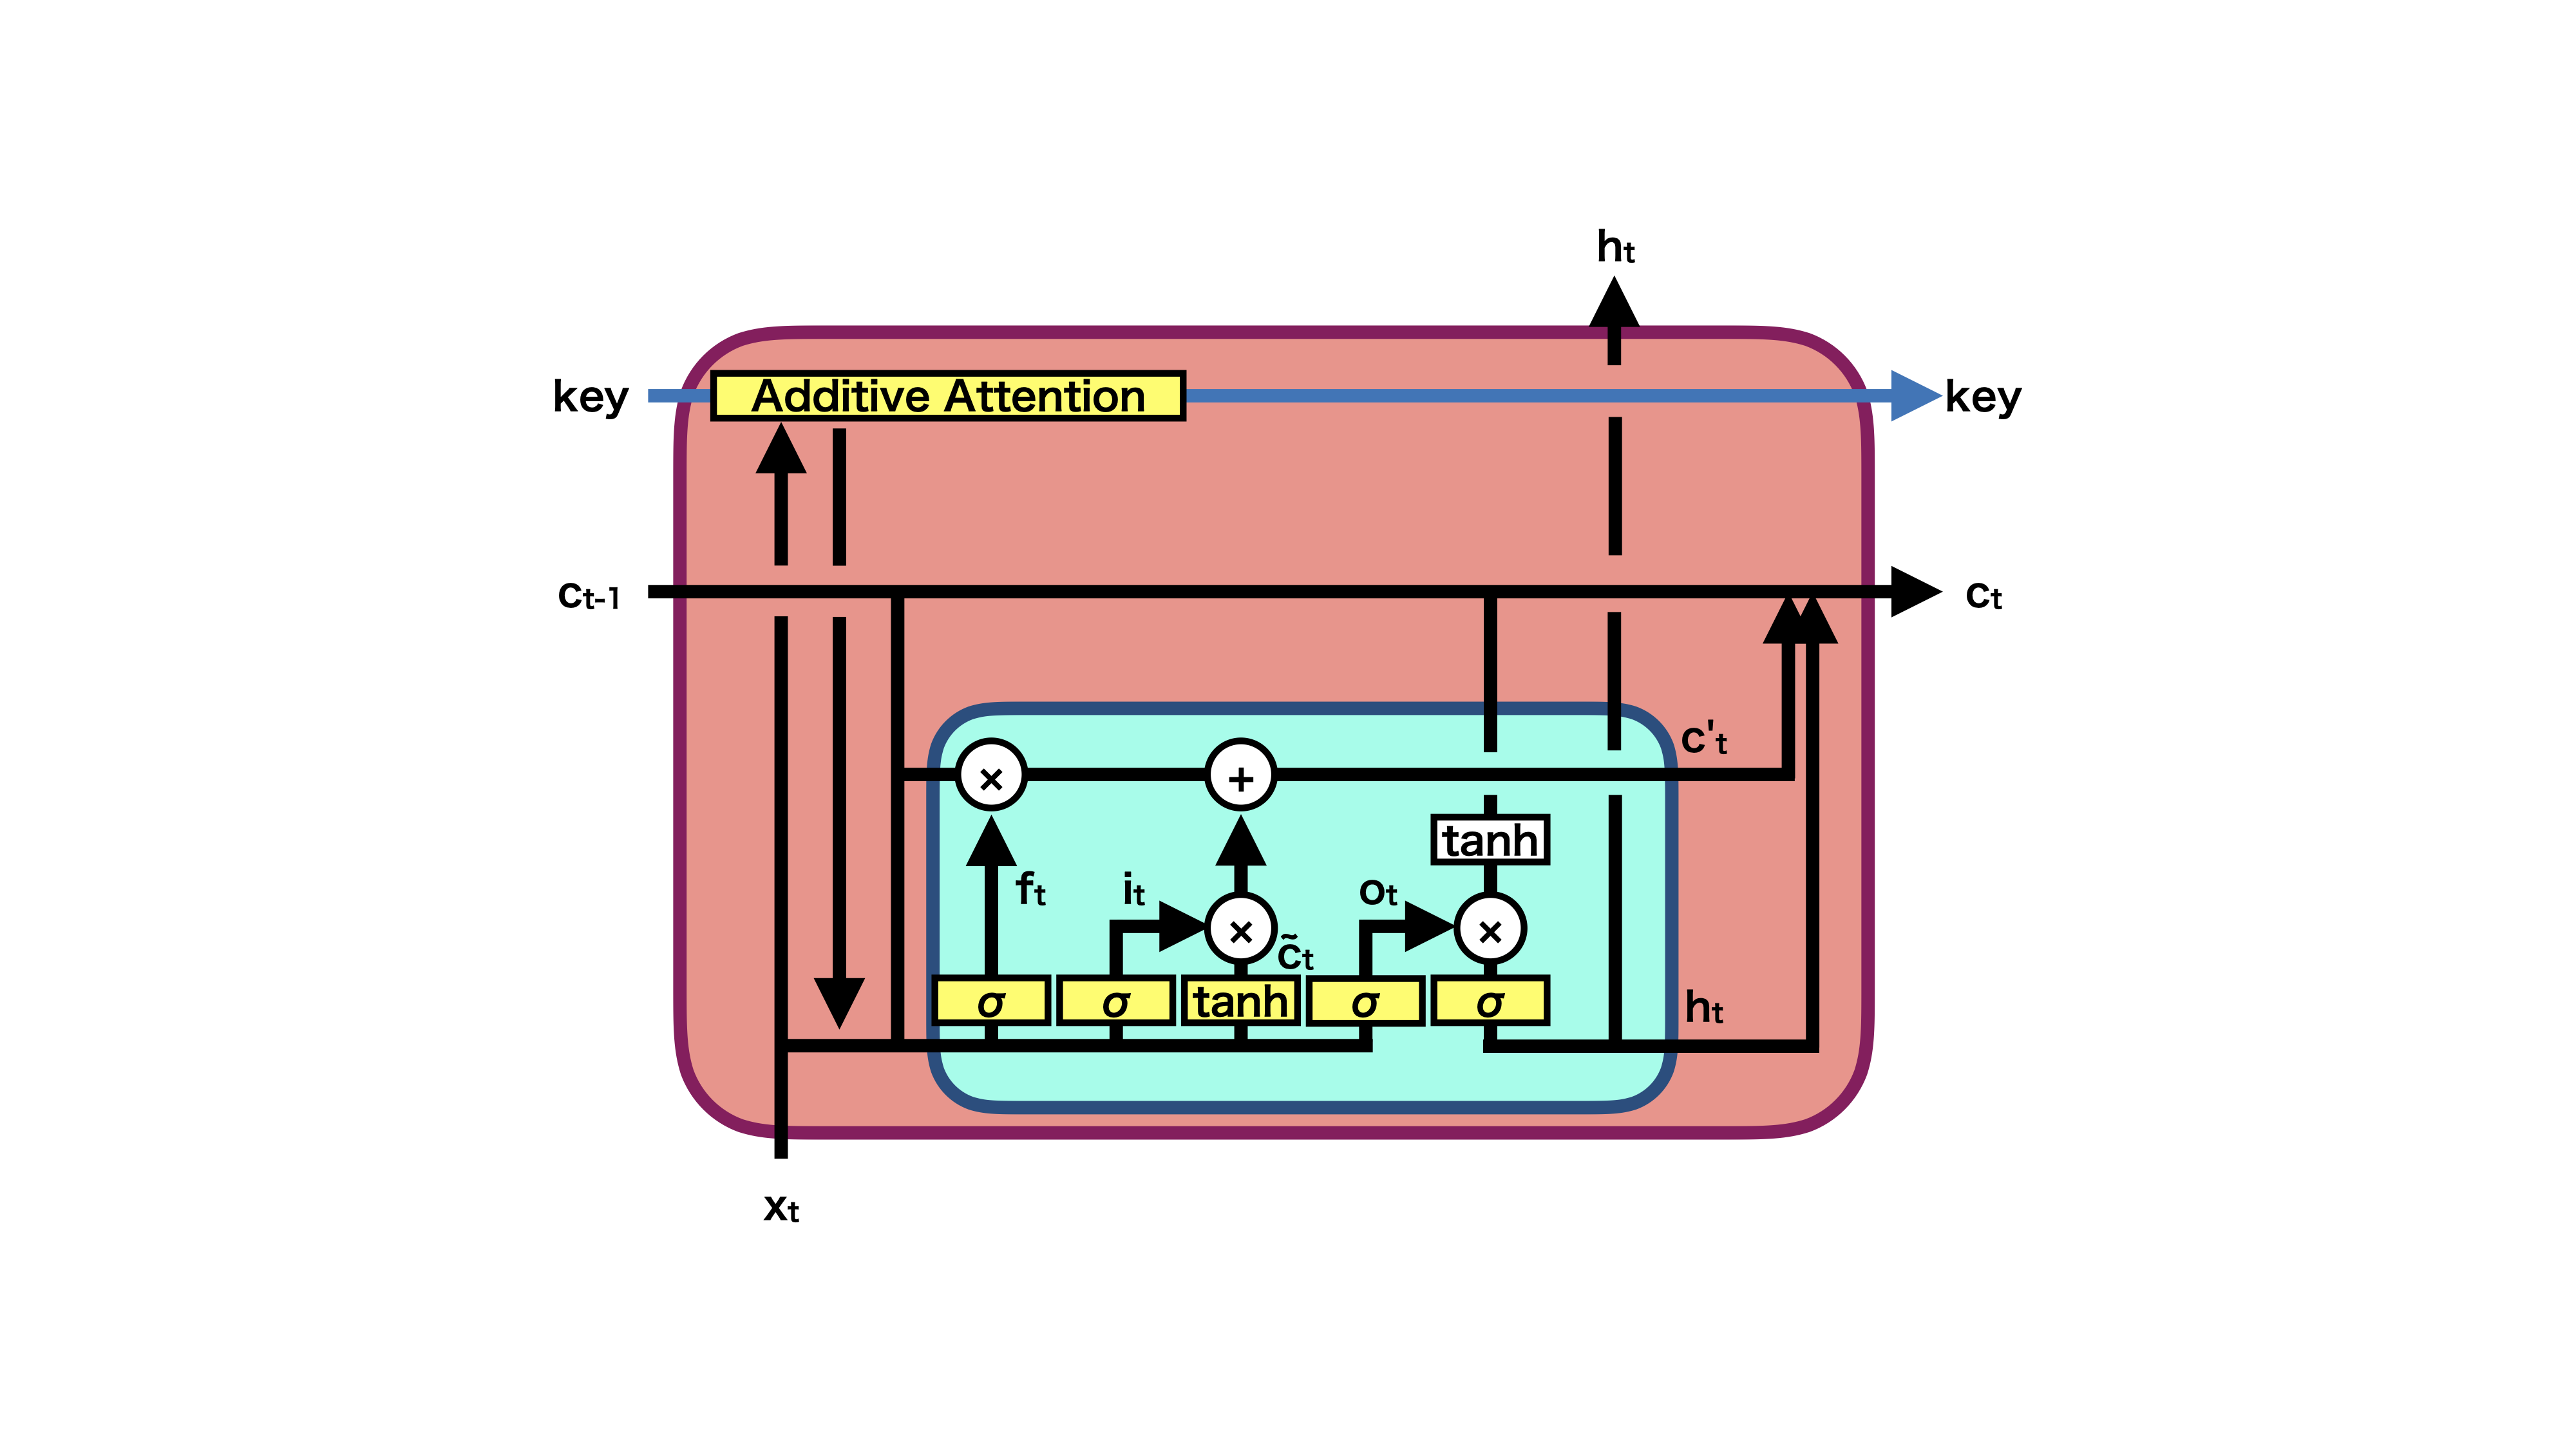
\includegraphics[width=0.9\textwidth]{Figure/3Networks/3-4-2-2AttentionVLSTM.png}
 \caption{Attentionを組み込んだ自作リカレントニューラルネットワークの構造}
 \label{3-4-2-2AttentionVLSTM}
\end{figure}


%%%%%%%%%%%%%%%%%%%%%%%%%%%%%%%%%%%%%%%%%%%%%%%%%%%%%%%%%%%%%%%%%%%%%%%%
\subsection{ネットワークの学習と戦略} \label{Net:VLSTM:TrainingandStrategyofVLSTM}

%%%%%%%%%%%%%%%%%%%%%%%%%%%%%%%%%%%%%%%%%%%%%%%%%%%%%%%%%%%%%%%%%%%%%%%%
\subsection{ネットワークの性能} \label{Net:VLSTM:PerformanceofVLSTM}

